% Document/LinearAlgebra/VectorSpaces/Foundations/Bases.tex
% Section: Bases and Dimension

\newpage
\section{Bases and Dimension}

\begin{definition}[Basis]\label{def:basis}
    Let $V$ be a $K$-vector space. A subset $B \subseteq V$ is a \textbf{basis} for $V$ if
    $B$ is both linearly independent and a generating system for $V$.

    A basis of infinite cardinality is sometimes called a \textbf{Hamel basis} to distinguish
    it from topological bases used in functional analysis.
\end{definition}

\begin{example}[Standard Bases]\label{ex:standard-bases}
    Consider the following examples of bases:
    \begin{enumerate}
        \item $\{(1, 0), (0, 1)\}$ is the standard basis for $\bb{R}^2$
        \item $\{(1, 1), (1, -1)\}$ is a non-standard basis for $\bb{R}^2$
        \item $\{1, X, X^2, \ldots\}$ is a basis for $K[X]$
        \item $\{e_1, \ldots, e_n\}$ is the standard basis for $K^n$
    \end{enumerate}

    \begin{center}
    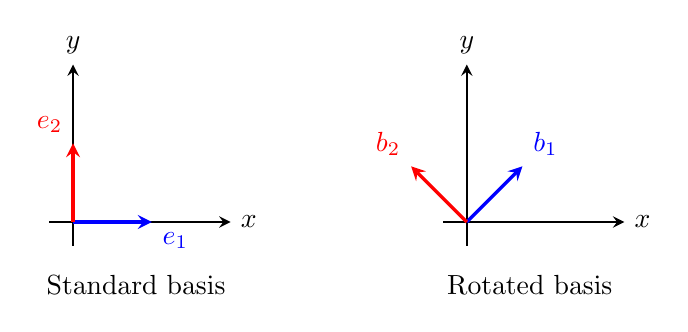
\begin{tikzpicture}[scale=1.0, >=stealth]
        % Standard basis
        \begin{scope}
            \draw[->, thick] (-0.3,0) -- (2,0) node[right] {$x$};
            \draw[->, thick] (0,-0.3) -- (0,2) node[above] {$y$};
            \draw[->, very thick, blue] (0,0) -- (1,0) node[below right] {$e_1$};
            \draw[->, very thick, red] (0,0) -- (0,1) node[above left] {$e_2$};
            \node at (0.8,-0.8) {Standard basis};
        \end{scope}

        % Rotated basis
        \begin{scope}[xshift=5cm]
            \draw[->, thick] (-0.3,0) -- (2,0) node[right] {$x$};
            \draw[->, thick] (0,-0.3) -- (0,2) node[above] {$y$};
            \draw[->, very thick, blue] (0,0) -- (0.707,0.707) node[above right] {$b_1$};
            \draw[->, very thick, red] (0,0) -- (-0.707,0.707) node[above left] {$b_2$};
            \node at (0.8,-0.8) {Rotated basis};
        \end{scope}
    \end{tikzpicture}
    \end{center}
\end{example}

\begin{example}[Bases in $\bb{R}^3$]\label{ex:bases-R3}
    In $\bb{R}^3$, consider the following:

    \textbf{Bases (linearly independent + spanning)}:
    \begin{itemize}
        \item $\{e_1, e_2, e_3\} = \{(1,0,0), (0,1,0), (0,0,1)\}$ --- standard basis
        \item $\{(1,1,0), (1,0,1), (0,1,1)\}$ --- non-standard basis (verify: determinant $\neq 0$)
        \item $\{(1,0,0), (1,1,0), (1,1,1)\}$ --- upper triangular basis
    \end{itemize}

    \textbf{Not a basis (spanning but dependent)}:
    \begin{itemize}
        \item $\{e_1, e_2, e_3, (1,1,1)\}$ --- 4 vectors in $\bb{R}^3$, so dependent
    \end{itemize}

    \textbf{Not a basis (independent but not spanning)}:
    \begin{itemize}
        \item $\{e_1, e_2\}$ --- only spans the $xy$-plane, not all of $\bb{R}^3$
    \end{itemize}

    \begin{center}
    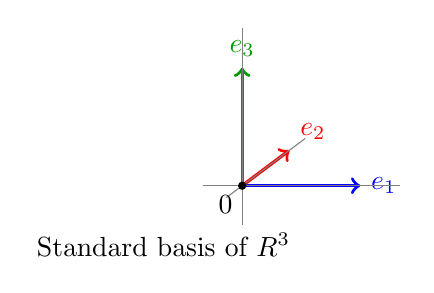
\begin{tikzpicture}[scale=1.0,
        x={(1cm,0cm)},
        y={(0.4cm,0.3cm)},
        z={(0cm,1cm)}]

        % Standard basis in R^3
        \draw[->, very thick, blue] (0,0,0) -- (1.5,0,0) node[right] {$e_1$};
        \draw[->, very thick, red] (0,0,0) -- (0,1.5,0) node[above right] {$e_2$};
        \draw[->, very thick, green!60!black] (0,0,0) -- (0,0,1.5) node[above] {$e_3$};

        % Coordinate axes (lighter)
        \draw[thin, gray] (-0.5,0,0) -- (2,0,0);
        \draw[thin, gray] (0,-0.5,0) -- (0,2,0);
        \draw[thin, gray] (0,0,-0.5) -- (0,0,2);

        \fill (0,0,0) circle (1.5pt) node[below left] {$0$};
        \node at (0,-2.5,0) {Standard basis of $\bb{R}^3$};
    \end{tikzpicture}
    \end{center}
\end{example}

\begin{proposition}[Basis as Direct Sum Decomposition]\label{prop:basis-direct-sum}
    $B$ is a basis for $V$ if and only if $V = \DirectSum{v \in B}{\Span[K]{\{v\}}}$.
\end{proposition}

\begin{proof}
    By Proposition~\ref{prop:lin-indep-direct-sum}, $B$ is linearly independent iff
    $(\Span[K]{\{v\}})_{v \in B}$ is a direct sum family.

    Moreover, $B$ generates $V$ iff $V = \Span[K]{B} = \SubspaceSum{v \in B}{\Span[K]{\{v\}}}$.

    Combining: $B$ is a basis iff the family is a direct sum family with sum $V$.
\end{proof}

\begin{remark}[Observations from Previous Sections]
    From our earlier work:
    \begin{itemize}
        \item The empty set $\emptyset$ is always linearly independent (Proposition~\ref{prop:empty-lin-indep})
        \item The whole space $V$ is always a generating system ($\Span[K]{V} = V$)
    \end{itemize}
\end{remark}

\begin{proposition}[Maximal/Minimal Characterizations]\label{prop:basis-maxmin}
    Let $V$ be a $K$-vector space. Then:
    \begin{enumerate}
        \item A linearly independent set is maximal (under inclusion) iff it is a basis
        \item A generating set is minimal (under inclusion) iff it is a basis
    \end{enumerate}
\end{proposition}

\begin{proof}
    \textbf{(1)}:

    ($\Rightarrow$)
    Let $L$ be maximal linearly independent. Suppose $L$ does not generate $V$.
    Then there exists $v \in V \setminus \Span[K]{L}$.
    By Proposition~\ref{prop:extend-lin-indep}, $L \Union \{v\}$ is linearly independent,
    contradicting maximality of $L$.

    ($\Leftarrow$)
    If $L$ is a basis, it is linearly independent. If $L \subsetneq M$ with $M$
    linearly independent, pick $v \in M \setminus L$. Since $L$ generates $V$, $v \in \Span[K]{L}$,
    so $M$ is not linearly independent by Proposition~\ref{prop:extend-lin-indep}. Contradiction.

    \textbf{(2)}:

    ($\Rightarrow$)
    Let $G$ be minimal generating. Suppose $G$ is linearly dependent.
    Then some $g \in G$ satisfies $g \in \Span[K]{G \setminus \{g\}}$.
    By Proposition~\ref{prop:span-properties}(7), $\Span[K]{G} = \Span[K]{G \setminus \{g\}}$,
    so $G \setminus \{g\}$ generates $V$, contradicting minimality.

    ($\Leftarrow$)
    If $G$ is a basis, it generates $V$. If $H \subsetneq G$ also generates $V$,
    pick $g \in G \setminus H$. Then $g \in \Span[K]{H} \subseteq \Span[K]{G \setminus \{g\}}$,
    contradicting linear independence.
\end{proof}

\begin{theorem}[Basis Extension Theorem]\label{thm:basis-extension}
    Let $L$ be a linearly independent subset and $G$ a generating set with $L \subseteq G$.
    Then there exists a basis $B$ with $L \subseteq B \subseteq G$.
\end{theorem}

\begin{proof}
    Consider the poset
    \[
        \mathcal{F} = \Set{M \mid L \subseteq M \subseteq G, M \text{ linearly independent}}
    \]
    ordered by inclusion. This is nonempty since $L \in \mathcal{F}$.

    \textbf{Chains have upper bounds}: Let $(M_\alpha)_{\alpha \in A}$ be a chain in $\mathcal{F}$.
    Set $M = \BigUnion[\alpha \in A] M_\alpha$. Then:
    \begin{itemize}
        \item $L \subseteq M \subseteq G$ since each $M_\alpha$ satisfies this.
        \item $M$ is linearly independent: any finite subset $F \subseteq M$ is contained in some $M_\alpha$
              (since chains are totally ordered), hence $F$ is linearly independent.
    \end{itemize}
    Thus $M \in \mathcal{F}$ is an upper bound.

    By Zorn's Lemma, $\mathcal{F}$ has a maximal element $B$.

    \textbf{$B$ is a basis}: $B$ is linearly independent by construction. We show $B$ generates $V$.
    Suppose $g \in G \setminus \Span[K]{B}$. Then $B \Union \{g\}$ is linearly independent
    (Proposition~\ref{prop:extend-lin-indep}) and satisfies $L \subseteq B \Union \{g\} \subseteq G$,
    contradicting maximality. Thus $G \subseteq \Span[K]{B}$, so $V = \Span[K]{G} \subseteq \Span[K]{B}$.
\end{proof}

\begin{corollary}[Fundamental Corollaries of Basis Extension]\label{cor:basis-extension}
    The following hold for any $K$-vector space $V$:
    \begin{enumerate}
        \item \textbf{Existence}: Every vector space has a basis (take $L = \emptyset$, $G = V$)
        \item \textbf{Extension}: Any linearly independent set can be extended to a basis (take $G = V$)
        \item \textbf{Extraction}: Any generating set contains a basis (take $L = \emptyset$)
    \end{enumerate}
\end{corollary}

\begin{theorem}[Steinitz Exchange Lemma]\label{thm:steinitz}
    Let $L$ be linearly independent and $S$ a spanning set for $V$.
    Then there exists an injection $f: L \to S$ such that
    $(S \setminus \DirectImage{f}{L}) \Union L$ spans $V$.
\end{theorem}

\begin{proof}
    Consider the poset
    \[
        \mathcal{P} = \Set{(L_0, S_0) \mid L_0 \subseteq L, S_0 \subseteq S, \exists \text{ bijection } g: L_0 \to S_0,
        (S \setminus S_0) \Union L_0 \text{ spans } V}
    \]
    ordered by $(L_0, S_0) \leq (L_1, S_1)$ iff $L_0 \subseteq L_1$ and $S_0 \subseteq S_1$.
    This is nonempty since $(\emptyset, \emptyset) \in \mathcal{P}$ (with $S$ spanning).

    \textbf{Chains have upper bounds}: Let $(L_\alpha, S_\alpha)$ be a chain.
    Set $\bar{L} = \BigUnion[\alpha] L_\alpha$ and $\bar{S} = \BigUnion[\alpha] S_\alpha$.
    The bijections $g_\alpha: L_\alpha \to S_\alpha$ combine to a bijection $\bar{L} \to \bar{S}$.
    For spanning: any $v \in V$ is a finite linear combination from $(S \setminus S_\alpha) \Union L_\alpha$
    for some $\alpha$, hence from $(S \setminus \bar{S}) \Union \bar{L}$.

    By Zorn's Lemma, there exists a maximal element $(\bar{L}, \bar{S})$ with bijection $\bar{g}: \bar{L} \to \bar{S}$.

    \textbf{Claim: $\bar{L} = L$}. Suppose $u \in L \setminus \bar{L}$.
    Since $(S \setminus \bar{S}) \Union \bar{L}$ spans $V$:
    \[
        u = \sum_{\ell \in \bar{L}} a_\ell \ell + \sum_{s \in F} b_s s
    \]
    for some finite $F \subseteq S \setminus \bar{S}$.
    If all $b_s = 0$, then $u \in \Span[K]{\bar{L}} \subseteq \Span[K]{L \setminus \{u\}}$,
    contradicting linear independence of $L$.
    So some $b_{s_0} \neq 0$. Then:
    \[
        s_0 = \frac{1}{b_{s_0}}\left(u - \sum_{\ell} a_\ell \ell - \sum_{s \neq s_0} b_s s\right)
    \]
    Thus $(S \setminus (\bar{S} \Union \{s_0\})) \Union (\bar{L} \Union \{u\})$ spans $V$
    (we can express $s_0$ in terms of the others).
    Setting $L' = \bar{L} \Union \{u\}$ and $S' = \bar{S} \Union \{s_0\}$ with $g'(u) = s_0$
    extends our pair, contradicting maximality.

    Thus $\bar{L} = L$, and $f = \bar{g}: L \to \bar{S} \subseteq S$ is the required injection.
\end{proof}

\begin{corollary}[Cardinality Bound]\label{cor:card-bound}
    If $L$ is linearly independent and $S$ spans $V$, then $\Card{L} \leq \Card{S}$.
\end{corollary}

\begin{proof}
    The injection $f: L \to S$ from Theorem~\ref{thm:steinitz} gives $\Card{L} \leq \Card{S}$.
\end{proof}

\begin{remark}[Finite-Dimensional Case and Choice]
    If $V$ has a \textbf{finite} generating set, both the Basis Extension Theorem and
    Steinitz Exchange Lemma hold \textbf{without} the Axiom of Choice.
    Zorn's Lemma for finite posets reduces to exhaustive search and is provable in ZF.
\end{remark}

\begin{theorem}[Dimension Invariance]\label{thm:dim-invariance}
    Any two bases of a vector space $V$ have the same cardinality.
\end{theorem}

\begin{proof}
    Let $B_1$ and $B_2$ be bases for $V$.
    Since $B_1$ is linearly independent and $B_2$ spans, $\Card{B_1} \leq \Card{B_2}$.
    Since $B_2$ is linearly independent and $B_1$ spans, $\Card{B_2} \leq \Card{B_1}$.
    By Cantor-Bernstein, $\Card{B_1} = \Card{B_2}$.
\end{proof}

\begin{definition}[Dimension]\label{def:dimension}
    The \textbf{dimension} of a $K$-vector space $V$, denoted $\Dim[K]{V}$, is the common
    cardinality of all bases of $V$.

    For infinite-dimensional spaces, dimension is an actual cardinal number
    (e.g., $\aleph_0$, $\mathfrak{c}$), \textbf{not} simply ``$\infty$''.
\end{definition}

\begin{corollary}[Dimension Zero and Trivial Spaces]\label{cor:dim-zero}
    $\Dim[K]{V} = 0$ if and only if $V = \{0\}$.
\end{corollary}

\begin{proof}
    $V = \{0\}$ has basis $\emptyset$ with $\Card{\emptyset} = 0$.
    Conversely, if $\Dim[K]{V} = 0$, then every basis has $0$ elements, 
    so $\emptyset$ is a basis and $V = \Span[K]{\emptyset} = \{0\}$.
\end{proof}

\begin{corollary}[Subspace with Equal Dimension]\label{cor:subspace-equal-dim}
    If $U \Subspace[K] V$ with $V$ finite-dimensional and $\Dim[K]{U} = \Dim[K]{V}$, then $U = V$.
\end{corollary}

\begin{proof}
    Let $B$ be a basis for $U$. Then $\Card{B} = \Dim[K]{U} = \Dim[K]{V}$.
    Since $B$ is linearly independent in $V$ and $\Card{B} = \Dim[K]{V}$,
    $B$ is a maximal linearly independent set in $V$ (Proposition~\ref{prop:basis-maxmin}),
    hence a basis for $V$. Thus $V = \Span[K]{B} = U$.
\end{proof}

\begin{proposition}[Dimensions of Finite-Dimensional Spaces]\label{prop:dim-finite}
    The following hold:
    \begin{enumerate}
        \item $\Dim[K]{K^n} = n$, since $\{e_1, \ldots, e_n\}$ is a basis.
        \item $\Dim[K]{K[X]_{\leq n}} = n + 1$, since $\{1, X, \ldots, X^n\}$ is a basis.
        \item $\Dim[K]{\MatSpace{m}{n}[K]} = mn$, since the elementary matrices $E_{ij}$ form a basis.
    \end{enumerate}
\end{proposition}

\begin{proof}
    In each case, we exhibit a basis and count its elements.

    \textbf{(1)}: The standard vectors $e_i = (0, \ldots, 0, 1, 0, \ldots, 0)$ with $1$ in position $i$
    span $K^n$ (any $(a_1, \ldots, a_n) = \sum_{i=1}^n a_i e_i$) and are linearly independent
    (evaluate at position $i$ to see coefficient $a_i$ is determined).

    \textbf{(2)}: The monomials $1, X, \ldots, X^n$ span $K[X]_{\leq n}$ by definition.
    They are linearly independent: if $\sum_{i=0}^n a_i X^i = 0$ as polynomials, then all $a_i = 0$.

    \textbf{(3)}: The elementary matrices $E_{ij}$ (with $1$ in position $(i,j)$ and $0$ elsewhere)
    span $\MatSpace{m}{n}[K]$ (any matrix $A = \sum_{i,j} A_{ij} E_{ij}$) and are linearly independent
    (the $(i,j)$-entry determines the coefficient of $E_{ij}$). There are $mn$ such matrices.
\end{proof}

\begin{proposition}[Dimension of Polynomial Space]\label{prop:dim-poly}
    $\Dim[K]{K[X]} = \aleph_0$.
\end{proposition}

\begin{proof}
    The set $\{1, X, X^2, \ldots\}$ is a basis:
    \begin{itemize}
        \item \textbf{Spanning}: Every polynomial is a finite linear combination of monomials.
        \item \textbf{Linear independence}: If $\sum_{i=0}^n a_i X^i = 0$, then all $a_i = 0$
              (polynomials are equal iff all coefficients are equal).
    \end{itemize}
    This basis is countably infinite, so $\Dim[K]{K[X]} = \Card{\bb{N}} = \aleph_0$.
\end{proof}

\begin{proposition}[Cardinality Comparisons]\label{prop:card-compare}
    For any $K$-vector space $V$:
    \begin{itemize}
        \item If $L$ is linearly independent, then $\Card{L} \leq \Dim[K]{V}$
        \item If $G$ generates $V$, then $\Dim[K]{V} \leq \Card{G}$
    \end{itemize}
\end{proposition}

\begin{proof}
    Immediate from Corollary~\ref{cor:card-bound} and the existence of a basis.
\end{proof}

\begin{theorem}[Grassmann Formula]\label{thm:grassmann}
    For subspaces $U, W \Subspace[K] V$:
    \[
        \Dim[K]{U + W} + \Dim[K]{U \Intersect W} = \Dim[K]{U} + \Dim[K]{W}
    \]
\end{theorem}

\begin{proof}
    Let $B_0$ be a basis for $U \Intersect W$.
    Extend $B_0$ to a basis $B_U$ for $U$ and to a basis $B_W$ for $W$
    (using Theorem~\ref{thm:basis-extension}).
    Write $B_U = B_0 \Union C_U$ and $B_W = B_0 \Union C_W$ (disjoint unions) where $C_U, C_W$ are the extension parts.

    \textbf{Claim}: $B_0 \Union C_U \Union C_W$ is a basis for $U + W$ (where the unions are disjoint).

    \textit{Spanning}: Any $u + w \in U + W$ with $u \in U$, $w \in W$ can be written as
    a linear combination of $B_U \Union B_W = B_0 \Union C_U \Union C_W$.

    \textit{Linear independence}: Suppose
    \[
        \sum_{b \in B_0} a_b b + \sum_{c \in C_U} a_c c + \sum_{d \in C_W} a_d d = 0
    \]
    The sum $v = \sum_{b \in B_0} a_b b + \sum_{c \in C_U} a_c c \in U$ equals
    $-\sum_{d \in C_W} a_d d \in W$.
    Thus $v \in U \Intersect W = \Span[K]{B_0}$.
    But $v = \sum_{b \in B_0} a_b b + \sum_{c \in C_U} a_c c$ with $C_U \Intersect B_0 = \emptyset$.
    By linear independence of $B_U = B_0 \Union C_U$, all $a_c = 0$.
    Thus $v = \sum_{b \in B_0} a_b b \in \Span[K]{B_0}$.
    Then $-\sum_{d \in C_W} a_d d = v \in \Span[K]{B_0}$.
    By linear independence of $B_W = B_0 \Union C_W$, all $a_d = 0$.
    Finally, $\sum_{b \in B_0} a_b b = 0$ implies all $a_b = 0$ by linear independence of $B_0$.

    Now count:
    \begin{align*}
        \Dim[K]{U + W} &= \Card{B_0} + \Card{C_U} + \Card{C_W} \\
        \Dim[K]{U} &= \Card{B_0} + \Card{C_U} \\
        \Dim[K]{W} &= \Card{B_0} + \Card{C_W} \\
        \Dim[K]{U \Intersect W} &= \Card{B_0}
    \end{align*}
    Adding: $\Dim[K]{U + W} + \Dim[K]{U \Intersect W} = 2\Card{B_0} + \Card{C_U} + \Card{C_W} = \Dim[K]{U} + \Dim[K]{W}$.
\end{proof}

\begin{corollary}[Direct Sum Dimension]\label{cor:direct-sum-dim}
    If $U \Intersect W = \{0\}$, then $\Dim[K]{U \DirectSum W} = \Dim[K]{U} + \Dim[K]{W}$.
\end{corollary}

\begin{proof}
    From Grassmann with $\Dim[K]{U \Intersect W} = \Dim[K]{\{0\}} = 0$.
\end{proof}

\begin{proposition}[Basis Union Lemma]\label{prop:basis-union}
    If $(U_i)_{i \in I}$ is a direct sum family and $B_i$ is a basis for $U_i$, then
    $\BigUnion[i \in I] B_i$ is a basis for $\DirectSum{i \in I}{U_i}$.
\end{proposition}

\begin{proof}
    \textbf{Spanning}: Each $u_i \in U_i$ is in $\Span[K]{B_i}$, so any finite sum $\sum_{i \in F} u_i$ (with $F \subseteq I$ finite) is in $\Span[K]{\BigUnion[i \in I] B_i}$.

    \textbf{Linear independence}: By Proposition~\ref{prop:direct-sum-lin-indep}, the union of linearly
    independent sets from a direct sum family is linearly independent.
\end{proof}

\begin{corollary}[Arbitrary Direct Sum Dimension]\label{cor:arbitrary-direct-dim}
    For a direct sum decomposition:
    \[
        \Dim[K]{\DirectSum{i \in I}{U_i}} = \sum_{i \in I} \Dim[K]{U_i}
    \]
    (where the sum is cardinal addition for infinite families).
\end{corollary}

\begin{theorem}[Inclusion-Exclusion for Dimension]\label{thm:dim-inclusion-exclusion}
    For a finite family $(U_1, \ldots, U_n)$ of subspaces:
    \[
        \Dim[K]{\sum_{i=1}^n U_i} = \sum_{\emptyset \neq J \subseteq \{1,\ldots,n\}} (-1)^{|J|+1} \Dim[K]{\BigIntersect[j \in J] U_j}
    \]
\end{theorem}

\begin{proof}
    By induction on $n$. The base case $n = 2$ is the Grassmann formula.

    For the inductive step, apply Grassmann to $U_n$ and $\sum_{i=1}^{n-1} U_i$, then use the
    identity $U_n \Intersect \sum_{i=1}^{n-1} U_i = \sum_{i=1}^{n-1} (U_n \Intersect U_i)$ (which holds for
    subspaces of an ambient space).
\end{proof}

\begin{theorem}[Cardinal Properties of Vector Spaces]\label{thm:cardinal-properties}
    Let $V \neq \{0\}$ be a non-trivial $K$-vector space with basis $B$. Then:
    \begin{enumerate}
        \item \textbf{Lower bound}: $\max(\Card{K}, \Card{B}) \leq \Card{V}$
        \item \textbf{Bijection with disjoint union}: There is a bijection
              \[
                  V \sim \BigUnion[n \in \bb{N}] (K \setminus \{0\})^n \times \binom{B}{n}
              \]
              where the union is disjoint. Thus:
              \[
                  \Card{V} = \sum_{n \in \bb{N}} (\Card{K} - 1)^n \cdot \binom{\Card{B}}{n}
              \]
        \item \textbf{Finite case}: If $\Card{B} = m$ is finite, then $\Card{V} = \Card{K}^m$.
        \item \textbf{Infinite case}: If $\max(\Card{K}, \Card{B}) = \kappa \geq \aleph_0$, then $\Card{V} = \kappa$.
    \end{enumerate}
\end{theorem}

\begin{proof}
    \textbf{(1)}: The map $k \mapsto k \cdot b_0$ embeds $K$ into $V$ for any fixed $b_0 \in B$.
    The map $b \mapsto 1 \cdot b$ embeds $B$ into $V$.

    \textbf{(2)}: We construct an explicit bijection. Let $v \in V$. Since $B$ is a basis,
    there exists a \textbf{unique} finite subset $F_v \subseteq B$ (the \textbf{support} of $v$)
    and \textbf{unique nonzero} scalars $(a_b)_{b \in F_v}$ such that
    \[
        v = \sum_{b \in F_v} a_b \cdot b
    \]
    Define the map $\phi: V \to \BigUnion[n \in \bb{N}] (K \setminus \{0\})^n \times \binom{B}{n}$ by:
    \[
        \phi(v) = \left((a_b)_{b \in F_v}, F_v\right) \in (K \setminus \{0\})^{|F_v|} \times \binom{B}{|F_v|}
    \]
    where $|F_v| = n$ is the size of the support.

    \textit{Injectivity}: If $\phi(v) = \phi(w)$, then $F_v = F_w$ and $(a_b)_{b \in F_v} = (c_b)_{b \in F_w}$,
    so $v = \sum_{b \in F_v} a_b b = \sum_{b \in F_w} c_b b = w$.

    \textit{Surjectivity}: Given $(a_1, \ldots, a_n) \in (K \setminus \{0\})^n$ and $\{b_1, \ldots, b_n\} \in \binom{B}{n}$,
    define $v = \sum_{i=1}^{n} a_i b_i$. Then $\phi(v) = ((a_1, \ldots, a_n), \{b_1, \ldots, b_n\})$.

    The union is disjoint because vectors have a unique support size. Taking cardinalities:
    \[
        \Card{V} = \sum_{n \in \bb{N}} \Card{(K \setminus \{0\})^n} \cdot \Card{\binom{B}{n}} = \sum_{n \in \bb{N}} (\Card{K} - 1)^n \cdot \binom{\Card{B}}{n}
    \]

    \textbf{(3)}: When $B$ is finite with $\Card{B} = m$, we have $\binom{m}{n} = 0$ for $n > m$.
    By the binomial theorem:
    \[
        \Card{V} = \sum_{n=0}^{m} (\Card{K} - 1)^n \cdot \binom{m}{n} = ((\Card{K} - 1) + 1)^m = \Card{K}^m
    \]

    \textbf{(4)}: Let $\kappa = \max(\Card{K}, \Card{B}) \geq \aleph_0$. From (2):
    \[
        \Card{V} = \sum_{n \in \bb{N}} (\Card{K} - 1)^n \cdot \binom{\Card{B}}{n} \leq \sum_{n \in \bb{N}} \kappa^n \cdot \kappa^n = \sum_{n \in \bb{N}} \kappa^{2n} = \aleph_0 \cdot \kappa = \kappa
    \]
    Combined with (1): $\kappa \leq \Card{V} \leq \kappa$, so $\Card{V} = \kappa$.
\end{proof}

\begin{proposition}[Infinite-Dimensional Examples]\label{prop:dim-infinite}
    The following are infinite-dimensional vector spaces with dimension $\mathfrak{c}$ (continuum):
    \begin{enumerate}
        \item $\Dim[\bb{Q}]{\bb{R}} = \mathfrak{c}$ (the reals as a $\bb{Q}$-vector space)
        \item $\Dim[\bb{R}]{C([0,1], \bb{R})} = \mathfrak{c}$ (continuous real functions on $[0,1]$)
    \end{enumerate}
\end{proposition}

\begin{proof}
    These results follow from the Cardinal Properties (Theorem~\ref{thm:cardinal-properties}).

    \textbf{(1)}: Let $B$ be a basis for $\bb{R}$ as a $\bb{Q}$-vector space.
    Since $\Card{\bb{Q}} = \aleph_0 < \mathfrak{c} = \Card{\bb{R}}$, we have $\Card{B} > \aleph_0$.
    By item (4) of Cardinal Properties with $\kappa = \max(\aleph_0, \Card{B}) = \Card{B}$:
    \[
        \Card{\bb{R}} = \Card{B}
    \]
    Since $\Card{\bb{R}} = \mathfrak{c}$, we have $\Dim[\bb{Q}]{\bb{R}} = \Card{B} = \mathfrak{c}$.

    \textbf{(2)}: We show $\mathfrak{c} \leq \Dim[\bb{R}]{C([0,1], \bb{R})} \leq \mathfrak{c}$.

    \textit{Upper bound}: The evaluation map $f \mapsto (f(q))_{q \in [0,1] \Intersect \bb{Q}}$
    embeds $C([0,1], \bb{R})$ into $\bb{R}^{\bb{Q} \Intersect [0,1]}$ (since continuous functions
    are determined by their values on a dense set). Thus:
    \[
        \Card{C([0,1], \bb{R})} \leq \Card{\bb{R}^{\bb{Q}}} = \mathfrak{c}^{\aleph_0} = \mathfrak{c}
    \]
    By Cardinal Properties (item 4), $\Dim[\bb{R}]{C([0,1], \bb{R})} \leq \mathfrak{c}$.

    \textit{Lower bound}: The functions $\{f_a : x \mapsto e^{ax} \mid a \in \bb{R}\}$
    are linearly independent (a nontrivial relation $\sum_{i=1}^n c_i e^{a_i x} = 0$
    with distinct $a_i$ would contradict the Wronskian being nonzero).
    Thus $\Dim[\bb{R}]{C([0,1], \bb{R})} \geq \mathfrak{c}$.
\end{proof}
